\section{Descrizione dei design pattern}
\label{DDP}

\subsection{Design pattern architetturali}
\subsubsection{MVC}
\paragraph{Contesto\\}
L'applicazione deve fornire una interfaccia grafica (GUI\glossario{}) costituita da più schermate, che mostrano vari dati all'utente. Inoltre, le informazioni che vengono visualizzate, devono essere sempre quelle aggiornate.

\paragraph{Problema\\}
L'applicazione deve avere una natura modulare e basata sulle responsabilità, al fine di ottenere una vera e propria applicazione component-based. Questo è conveniente per poter più facilmente gestire la manutenzione dell'applicazione.\\
Appare quindi chiaro il bisogno di un'architettura che permetta la separazione netta tra i componenti software che gestiscono il modo di presentare i dati, e i componenti che gestiscono i dati stessi.

\paragraph{Soluzione e struttura\\}
L'applicazione deve separare i componenti software che implementano il modello delle funzionalità di business, dai componenti che implementano la logica di presentazione e di controllo che utilizzano tali funzionalità. Vengono quindi definiti tre tipologie di componenti che soddisfano tali requisiti: 
\begin{itemize}
\item \textbf{Model:} implementa le funzionalità di business;
\item \textbf{View:} implementa la logica di presentazione;
\item \textbf{Controller:} implementa la logica di controllo.
\end{itemize}
La figura seguente ha lo scopo di offrire una rappresentazione della struttura del design pattern\glossario{} MVC.
\begin{figure} [!h]
	\centering
	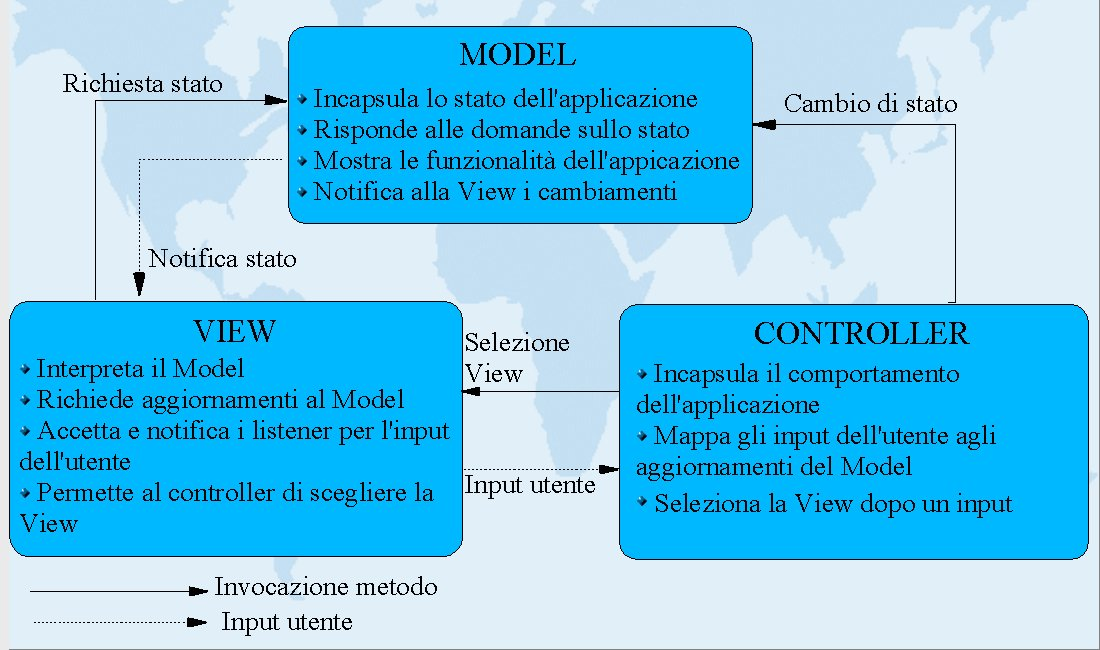
\includegraphics[width=\linewidth]{./Content/Immagini/mvc.jpg}
	\caption{Diagramma del design pattern MVC}
	\label{figMVC}
\end{figure}

\paragraph{Scopo\\}
Disaccoppiare le tre componenti.

\paragraph{Partecipanti e responsabilità}
\begin{itemize}
\item \textbf{Model:}
Analizzando la figura \ref{figMVC}, si evince che il core dell'applicazione viene implementato dal Model, che, incapsulando lo stato dell'applicazione, definisce i dati e le operazioni che possono essere eseguite su questi. Definisce quindi le regole di business per l'interazione con i dati, esponendo alla View ed al Controller rispettivamente le funzionalità per l'accesso e l'aggiornamento.\\
Per lo sviluppo del Model, è vivamente consigliato utilizzare le tipiche tecniche di progettazione object oriented, al fine di ottenere un componente software che astragga al meglio i concetti importati dal mondo reale. Il Model può inoltre avere la responsabilità di notificare ai componenti della View eventuali aggiornamenti verificatisi in seguito a richieste del Controller, al fine di permettere alle View di presentare agli occhi degli utenti dati sempre aggiornati;

\item \textbf{View:}
La logica di presentazione dei dati viene gestita solo e solamente dalla View. Ciò implica che questa deve fondamentalmente gestire la costruzione dell' interfaccia grafica (GUI\glossario{}), che rappresenta il mezzo mediante il quale gli utenti interagiranno con il sistema. Ogni GUI\glossario{} può essere costituita da schermate diverse che presentano più modi di interagire con i dati dell'applicazione. Per far sì che i dati presentati siano sempre aggiornati, è possibile adottare due strategie note come \lq\lq{}push model\rq\rq{} e \lq\lq{}pull model\rq\rq{}.\\
Il push model adotta il pattern Observer, registrando le View come osservatori del Model. Le View possono quindi richiedere gli aggiornamenti al Model in tempo reale, grazie alla notifica di quest'ultimo. Benché questa rappresenti la strategia ideale, non è sempre applicabile. In tali casi è possibile utilizzare il \lq\lq{}pull Model\rq\rq{}, dove la View richiede gli aggiornamenti quando \lq\lq{}lo ritiene opportuno\rq\rq{}. Inoltre, la View delega al Controller l'esecuzione dei processi richiesti dall'utente, dopo averne catturato gli input e la scelta delle eventuali schermate da presentare;

\item \textbf{Controller:}
Questo componente ha la responsabilità di trasformare le interazioni dell'utente con la View, in azioni eseguite dal Model. Il Controller non rappresenta un semplice \lq\lq{}ponte\rq\rq{} tra View e Model. Realizzando la mappatura tra input dell'utente e processi eseguiti dal Model e selezionando la schermate della View richieste, il Controller implementa la logica di controllo dell'applicazione.
\end{itemize}

\paragraph{Applicabilità\\}
Il design pattern\glossario{} MVC\glossario{} può essere utilizzato nei seguenti casi:
\begin{itemize}
\item Quando si vuole trattare un gruppo di oggetti come un oggetto singolo;
\item Quando si vuole disaccoppiare View e Model instaurando un protocollo di sottoscrizione e notifica tra loro;
\item Quando si vogliono agganciare più View a un Model per fornire più rappresentazioni del Model stesso.
\end{itemize} 
\pagebreak

\subsection{Design pattern creazionali}
\label{DPC}
\subsubsection{Factory}
\label{Factory}
\begin{figure} [!h]
	\centering
	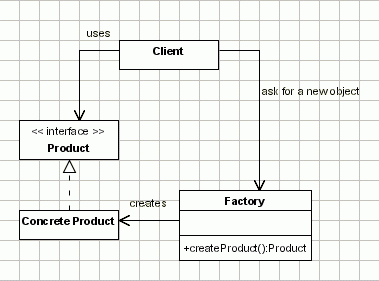
\includegraphics[width=0.5\linewidth]{./Content/Immagini/Factory.png}
	\caption{Diagramma del design pattern Factory}
	\label{figFact}
\end{figure}

\paragraph{Scopo\\}
Definire un'interfaccia per la creazione di un oggetto, lasciando alle sottoclassi la decisione sulla classe che deve essere istanziata. Il design pattern\glossario{} Factory consente di deferire l'istanziazione di una classe alle sottoclassi.

\paragraph{Motivazione\\}
I framework\glossario{} utilizzano classi astratte per definire e mantenere le relazioni tra oggetti e spesso sono anche responsabili della creazione di questi oggetti. Il framework\glossario{} deve gestire l'istanziazione di classi, ma ha conoscenza diretta soltanto di classi astratte, che non possono essere istanziate. il pattern fornisce una soluzione a questo problema; incapsula la conoscenza su quale specifica sottoclasse deve essere creata e sposta questa conoscenza all'esterno del framework\glossario{}. Factory è una variante del design pattern\glossario{} Factory Method.

\paragraph{Implementazione\\}
Il client ha bisogno di un Concrete Product, ma invece di crearlo direttamente con l'uso dell'operatore "new" chiede di crearlo all'oggetto Factory dandogli informazioni sul tipo di oggetto da creare.
Il Factory istanzia un nuovo concrete Product e ritorna al client il prodotto appena creato (facendo un cast alla classe astratta Product);
Il client usa i Concrete Product come Product senza essere conscio della loro concreta implementazione.
\pagebreak

\subsubsection{Singleton}
\label{single}
\begin{figure} [!h]
	\centering
	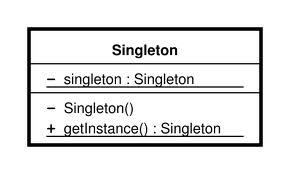
\includegraphics[width=0.43\linewidth]{./Content/Immagini/singleton.jpg}
	\caption{Diagramma del design pattern Singleton}
	\label{figSing}
\end{figure}

\paragraph{Scopo\\}
Assicurare che una classe abbia una sola istanza e fornire un punto d'accesso globale a tale istanza.

\paragraph{Motivazione\\}
È importante poter assicurare che per alcune classi esista una sola istanza. Per raggiungere questo scopo, la classe stessa ha la responsabilità di creare le proprie istanze, assicurare che nessun'altra istanza possa essere creata e fornire un modo semplice per accedere all'istanza.

\paragraph{Applicabilità\\} 
Il design pattern\glossario{} Singleton può essere utilizzato nei seguenti casi:
\begin{itemize}
\item Quando deve esistere esattamente un'istanza di una classe e tale istanza deve essere resa accessibile ai client attraverso un punto di accesso noto a tutti gli utilizzatori;
\item Quando l'unica istanza deve poter essere estesa attraverso la definizione di sottoclassi e i client devono essere in grado di utilizzare le istanze estese, senza dover modificare il proprio codice.
\end{itemize}
\pagebreak

\subsection{Design pattern strutturali}
\subsubsection{Adapter}
\label{DPAda}
\begin{figure} [!h]
	\centering
	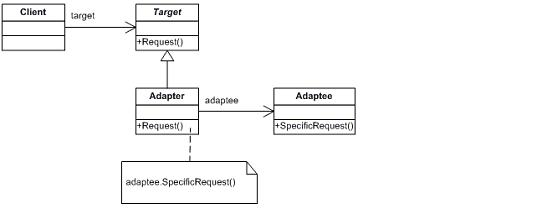
\includegraphics[width=\linewidth]{./Content/Immagini/adapter.jpg}
	\caption{Diagramma del design pattern Adapter}
	\label{figAda}
\end{figure}
\paragraph{Scopo\\}
Convertire l'interfaccia di una classe in un'altra interfaccia richiesta dal client. Esso consente a classi diverse di operare insieme, quando ciò non è altrimenti possibile a causa di interfacce incompatibili.

\paragraph{Motivazione\\}
A volte, una classe di supporto che è stata progettata con obiettivi di riuso, non può essere riusata, semplicemente perché la sua interfaccia non è compatibile con l'interfaccia richiesta da un'applicazione.

\paragraph{Applicabilità\\}
Il design pattern\glossario{} Adapter può essere utilizzato nei seguenti casi:
\begin{itemize}
\item Quando si vuole usare una classe esistente, ma la sua interfaccia non è compatibile con quella desiderata;
\item Quando si vuole creare una classe riusabile in grado di cooperare con classi non correlate o impreviste, cioè con classi che non necessariamente hanno interfacce compatibili;
\item Per gli oggetti adapter quando si devono utilizzare diverse sottoclassi esistenti, ma non è pratico adattare la loro interfaccia creando una sottoclasse per ciascuna di esse.
\end{itemize}
\pagebreak

\subsubsection{DAO (Data Access Object)}
\label{DPDAO}
\begin{figure} [!h]
	\centering
	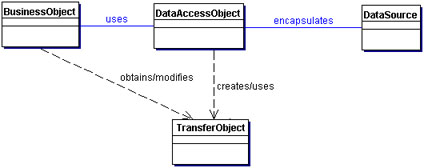
\includegraphics[width=0.7\linewidth]{./Content/Immagini/DAO.jpg}
	\caption{Diagramma del design pattern DAO}
	\label{figDao}
\end{figure}

\paragraph{Caratteristiche\\}
\begin{itemize}
\item Incapsula l'accesso ai dati;
\item Permette la sostituzione della tecnologia di memorizzazione senza modifiche al resto del programma;
\item Disaccoppia le entità dal relativo codice di persistenza.
\end{itemize}

\paragraph{Giustificazione\\}
L'utilizzo del design pattern\glossario{} DAO permette di ridurre le dipendenze fra logica di business e logica di persistenza, in quanto la comunicazione con il database, viene lasciata agli oggetti propri del design pattern\g{}, rendendo il sistema manutenibile.

\subsubsection{Proxy}
\label{DPProxy}
	\begin{figure}[!h]
		\centering
		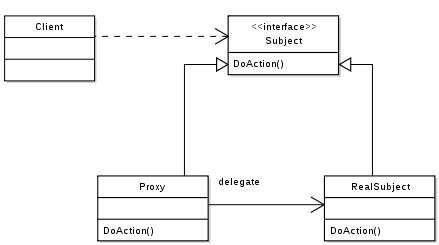
\includegraphics[width=\linewidth]{./Content/Immagini/proxydp.png}
		\caption{Diagramma del design pattern Proxy}
		\label{figproxy}
	\end{figure}
	
	\paragraph{Scopo\\}
	Fornire un surrogato o un segnaposto di un altro oggetto per controllare l'accesso a tale oggetto.
	
	\paragraph{Motivazione\\}
	Una ragione per effettuare un controllo sull'accesso a un oggetto può essere quella di rinviare il costo della sua creazione e inizializzazione fino a quando l'oggetto non è effettivamente necessario.	
	\paragraph{Applicabilità\\}
	Il design pattern\glossary{} è applicabile nelle seguenti situazioni:
	\begin{itemize}
		\item Un proxy remoto fornisce un rappresentante local per un oggetto in diverso spazio di indirizzamento;
		\item Un proxy virtuale gestisce la creazione su richiesta di oggetti \lq\lq{}costosi\rq\rq{};
		\item Un proxy di protezione controlla l'accesso a un oggetto. Questo tipo di proxy si rivela utile quando possono essere definiti diritti di accesso diversi per gli oggetti;
		\item Un riferimento intelligente sostituisce un puntatore puro ad un oggetto, consentendo l'esecuzione di attività aggiuntive quando si accede all'oggetto referenziato.
	\end{itemize}
\pagebreak

\subsection{Design pattern comportamentali}
\subsubsection{Strategy}
\label{DPStrategy}
\begin{figure}[!h]
	\centering
	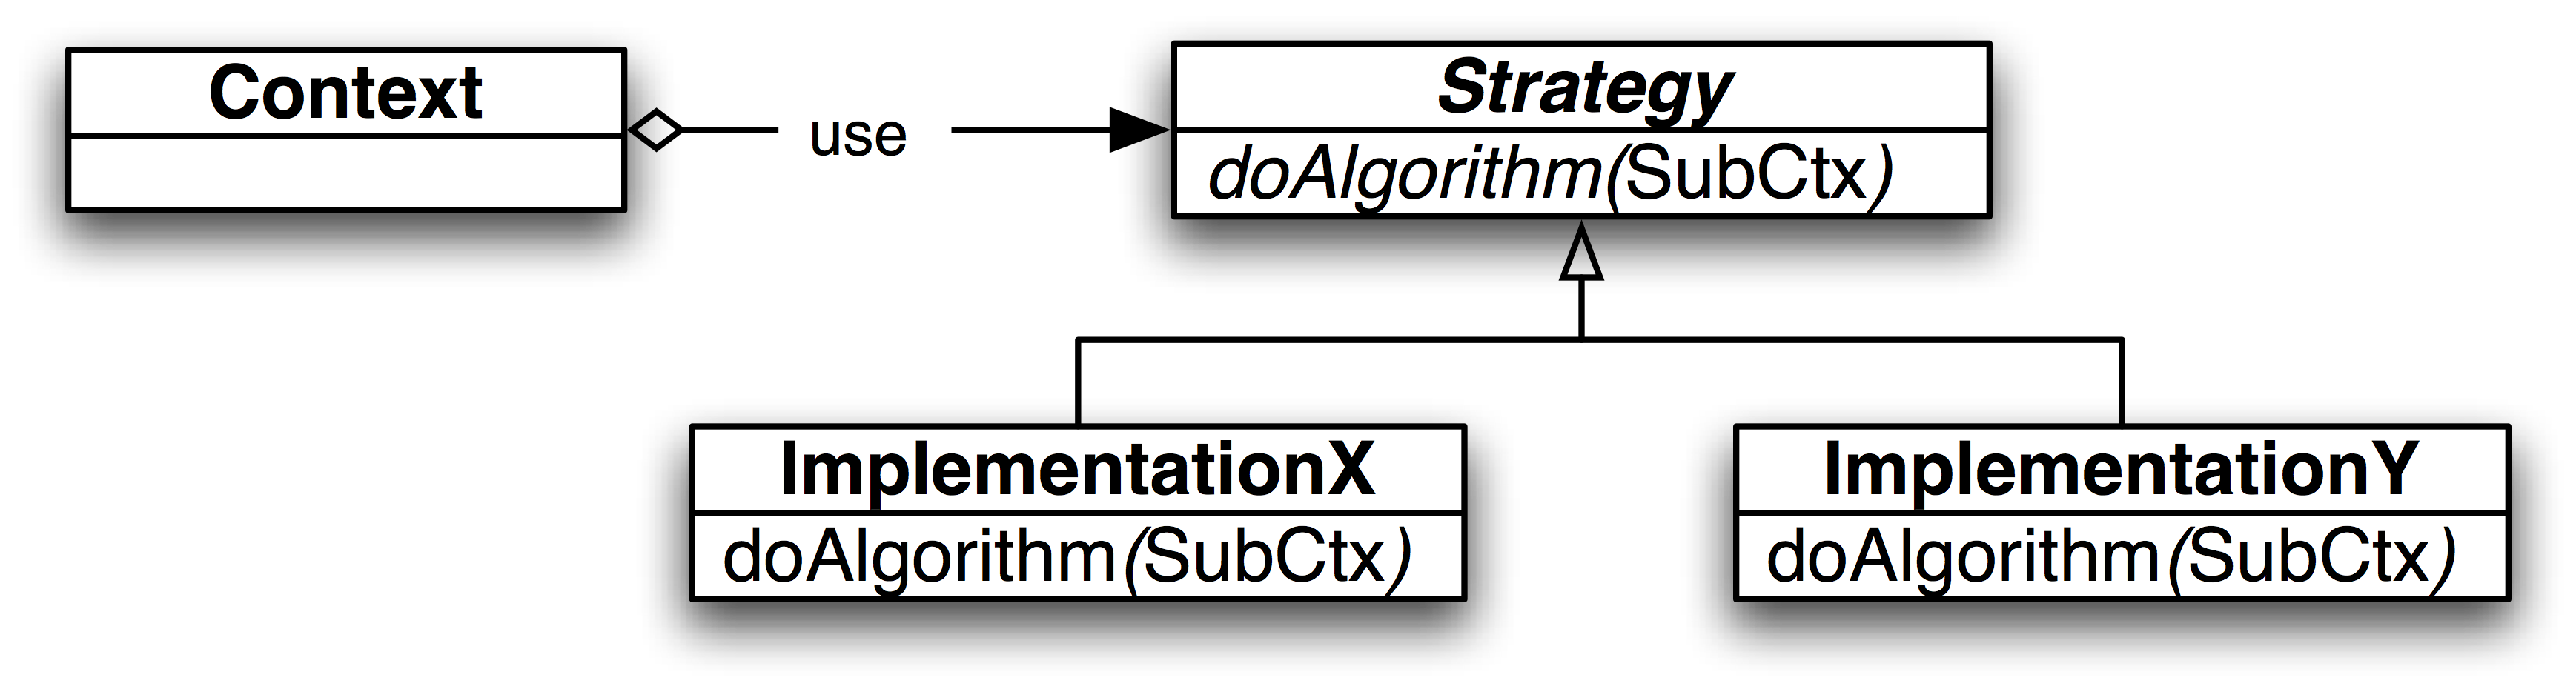
\includegraphics[width=0.7\linewidth]{./Content/Immagini/Strategy.png}
	\caption{Diagramma del design pattern Strategy}
	\label{figStra}
\end{figure}

\paragraph{Scopo\\}
Definire una famiglia di algoritmi, incapsularli e renderli intercambiabili. Permette agli algoritmi di variare indipendentemente dai client che ne fanno uso.

\paragraph{Motivazione\\}
Esistono molti algoritmi (strategie) che non possono essere inserite direttamente nei client:
\begin{itemize}
\item I client rischiano di essere troppo complessi;
\item Differenti strategie sono appropriate in casi differenti;
\item Difficoltà nell'aggiungere nuovi algoritmi e modificare gli esistenti.
\end{itemize}

\paragraph{Applicabilità\\}
Il design pattern\glossario{} Strategy può essere utilizzato nei seguenti casi:
\begin{itemize}
\item Implementare le parti invarianti di un algoritmo una volta sola;
\item Evitare la duplicazione del codice;
\item Controllare le possibili estensioni di una classe;
\item Un algoritmo usa una struttura dati che non dovrebbe essere resa nota ai client. Strategy può essere usato per evitare di esporre strutture dati complesse e specifiche dell'algoritmo.
\end{itemize}